\documentclass[10pt]{article}
\usepackage[letterpaper]{geometry}
\geometry{verbose,tmargin=1in,bmargin=1in,lmargin=1in,rmargin=1in}
\usepackage{setspace}
\usepackage{ragged2e}
\usepackage{color}
\usepackage{titlesec}
\usepackage{graphicx}
\usepackage{float}
\usepackage{mathtools}
\usepackage{amsmath}
\usepackage[font=small,labelfont=bf,labelsep=period]{caption}
\usepackage[english]{babel}
\usepackage{indentfirst}
\usepackage{array}
\usepackage{makecell}
\usepackage[usenames,dvipsnames]{xcolor}
\usepackage{multirow}
\usepackage{tabularx}
\usepackage{arydshln}
\usepackage{caption}
\usepackage{subcaption}
\usepackage{xfrac}
\usepackage{etoolbox}
\usepackage{cite}
\usepackage{url}
\usepackage{dcolumn}
\usepackage{hyperref}
\usepackage{courier}
\usepackage{url}
\usepackage{esvect}
\usepackage{commath}
\usepackage{verbatim} % for block comments
\usepackage{enumitem}
\usepackage{hyperref} % for clickable table of contents
\usepackage{braket}
\usepackage{titlesec}
\usepackage{booktabs}
\usepackage{gensymb}
\usepackage{longtable}
\usepackage{listings}
\usepackage{cancel}
\usepackage{tcolorbox}
\usepackage[mathscr]{euscript}
\lstset{
    frame=single,
    breaklines=true,
    postbreak=\raisebox{0ex}[0ex][0ex]{\ensuremath{\color{red}\hookrightarrow\space}}
}

% for circled numbers
\usepackage{tikz}
\newcommand*\circled[1]{\tikz[baseline=(char.base)]{
            \node[shape=circle,draw,inner sep=2pt] (char) {#1};}}


\titleclass{\subsubsubsection}{straight}[\subsection]

% define new command for triple sub sections
\newcounter{subsubsubsection}[subsubsection]
\renewcommand\thesubsubsubsection{\thesubsubsection.\arabic{subsubsubsection}}
\renewcommand\theparagraph{\thesubsubsubsection.\arabic{paragraph}} % optional; useful if paragraphs are to be numbered

\titleformat{\subsubsubsection}
  {\normalfont\normalsize\bfseries}{\thesubsubsubsection}{1em}{}
\titlespacing*{\subsubsubsection}
{0pt}{3.25ex plus 1ex minus .2ex}{1.5ex plus .2ex}

\makeatletter
\renewcommand\paragraph{\@startsection{paragraph}{5}{\z@}%
  {3.25ex \@plus1ex \@minus.2ex}%
  {-1em}%
  {\normalfont\normalsize\bfseries}}
\renewcommand\subparagraph{\@startsection{subparagraph}{6}{\parindent}%
  {3.25ex \@plus1ex \@minus .2ex}%
  {-1em}%
  {\normalfont\normalsize\bfseries}}
\def\toclevel@subsubsubsection{4}
\def\toclevel@paragraph{5}
\def\toclevel@paragraph{6}
\def\l@subsubsubsection{\@dottedtocline{4}{7em}{4em}}
\def\l@paragraph{\@dottedtocline{5}{10em}{5em}}
\def\l@subparagraph{\@dottedtocline{6}{14em}{6em}}
\makeatother

\newcommand{\volume}{\mathop{\ooalign{\hfil$V$\hfil\cr\kern0.08em--\hfil\cr}}\nolimits}

% Generate the glossary of acronyms
\usepackage[acronym]{glossaries}
\makeglossaries

\newacronym{ai}{AI}{Arithmetic Intensity}
\newacronym{avx}{AVX}{Advanced Vector Extensions}
\newacronym{blas}{BLAS}{Basic Linear Algebra Subroutines}
\newacronym{clump}{CLUMP}{Cluster of Symmetric Multiprocessor}
\newacronym{dram}{DRAM}{Dynamic Random Access Memory}
\newacronym{fma}{FMA}{Fused Multiply-Add}
\newacronym{gpu}{GPU}{Graphics Processing Unit}
\newacronym{ilp}{ILP}{Instruction Level Programming}
\newacronym{mpi}{MPI}{Message Passing Interface}
\newacronym{nersc}{NERSC}{National Energy Research Scientific Computing Center}
\newacronym{ni}{NI}{Network Interface}
\newacronym{simd}{SIMD}{Single Instruction, Multiple Data}
\newacronym{smp}{SMP}{Symmetric Multiprocessor}
\newacronym{sram}{SRAM}{Second Random Access Memory}
\newacronym{sse}{SSE}{Streaming SIMD Extensions}

\setcounter{secnumdepth}{4}
\setcounter{tocdepth}{4}
\begin{document}

\title{CS 267: HW 1}
\author{Kirk Larsen, James McCauley, April Novak}

\maketitle

\section{Introduction}

The purpose of this assignment is to optimize matrix-matrix multiplication to run as fast as possible on a single processor on the Edison machine at the \gls{nersc}. All methods used for optimizing matrix-matrix multiply pursued here will use \(2n^3\) (or more) floating point operations for matrices of size \(n\times n\). Hence, the methods used to optimize matrix-matrix multiplication will focus not on reducing the number of flops by using algorithms such as Strassen's method, but rather by reducing movement through the memory hierarchy. 

% put in more about Edison
Edison has 12 cores per CPU, with a 2.4 GHz AVX frequency. 

This report is organized into two main sections. The first section focuses on the naive implementation using three non-blocked loops. Various performance-improving techniques were first tested with this simpler code in order to guide the optimization performed with the blocked method. After discussing techniques that were used to speed up the naive implementation, the improvements upon the blocked algorithm are discussed. All major attempts to optimize the code, whether successful or unsuccessful, are discussed in order to show all results and conclude which actions have the greatest impact on performance on a serial processor. Finally, the final optimized code is run on a different machine, and conclusions are given.

\section{Naive Implementation}

This section discusses benchmark results obtained with the naive implementation ({\tt dgemm-naive.c}) of matrix-matrix multiply using three nested non-blocked loops. The innermost loop computes the dot product of a row of \(A\) with a column of \(B\), and assigns this to an entry in \(C\). 

\subsection{Register Encouragement}
The only attempt at some level of optimization in the as-provided code is the encouragement of the compiler in putting the intermediate value {\tt cij} in a register by defining this \textit{technically unnecessary} variable just outside the innermost loop. This causes {\tt cij} to be stored in a register for fast retrieval for all of the {\tt k} loops for a given {\tt i} and {\tt j}. This optimization can be shown by changing the original code block to the following, which removes any attempt to encourage the compiler to place {\tt C[i+j*n]} in a register and results in more slow memory operations. Fig. \ref{fig:1} shows the difference in Mflop/s for (a) the original code that encourages the compiler to place a frequently-used variable in a register and (b) code that removes the variable {\tt cij}.

\begin{lstlisting}[language=C, basicstyle=\small][H]
void square_dgemm (int n, double* A, double* B, double* C) {
  for (int i = 0; i < n; ++i) {
    for (int j = 0; j < n; ++j) {
      for(int k = 0; k < n; k++)
        C[i+j*n] += A[i+k*n] * B[k+j*n];
}}}
\end{lstlisting}

\begin{figure}[H]
\centering
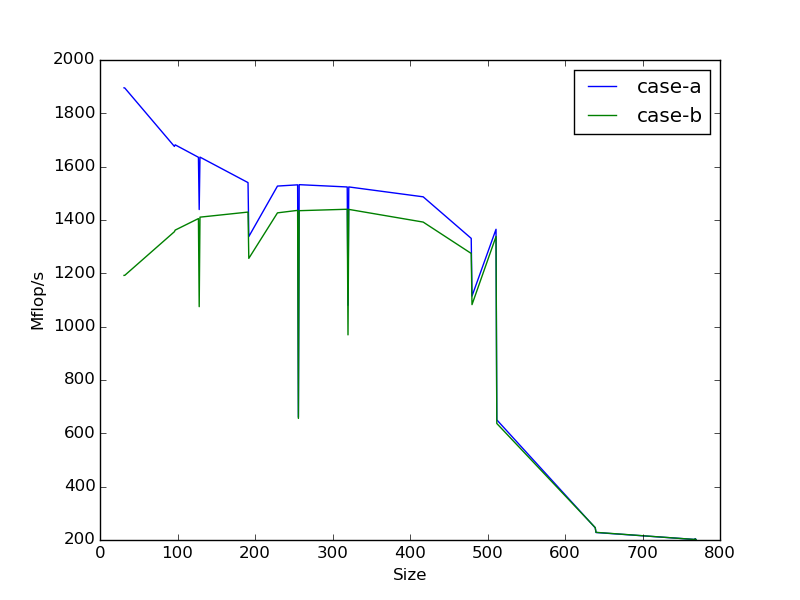
\includegraphics[width=0.6\textwidth]{figures/fig1.png}
\caption{Difference in Mflop/s for (a) the original code encouraging register-allocation for {\tt cij} and (b) the even-more naive code with greater slow memory traffic (no intermediate variable {\tt cij} defined).}
\label{fig:1}
\end{figure}

Encouraging the compiler to place commonly-used variables in the register offers the best improvement in speed for smaller matrix sizes. As can be seen from Fig. \ref{fig:1}, for matrices of size greater than about 500\(\times\)500, the improvement is negligible. This may be due to the fact that other processes in the algorithm begin to dominate and bottleneck, rather than the slow memory access of {\tt C[i+j*n]}. These other processes can be calls to memory locations further and further from the chip as the matrix size increases beyond the successive cache sizes. This technique of encouraging the compiler to place variables in a register is applicable for the blocked algorithm discussed in the next section, and hence will be used in the {\tt do\_block} routine.

% Did I interpret those dips correctly?
Fig. \ref{fig:1} also provides information regarding the memory structure of Edison. Both curves in Fig. \ref{fig:1} show very sharp dips in performance at matrix sizes of 128, 256, and 320, where the speed decreases monotonically after a size of 511. Because these dips in performance occur regardless of if the compiler is being encourage to store values in the register, they are likely due to the boundaries at which memory must first be retrieved from the L1-cache, L2-cache, L-3 cache, \gls{dram}, and so on.

\subsection{Matrix Layout}
A second way to attempt to optimize the naive algorithm is with the technique of copy optimization, where the layout of one or more matrices is copied to a new location and modified to take advantage of the order in which the data is used. For C, because arrays are stored in column-major layout, the indexing over the rows in \(A\) is slow, because large strides are taken between data retrieval such that each read is likely a cache miss. By transposing \(A\), and indexing instead over columns, the code should be able to perform matrix-matrix multiplication faster. Memory is allocated for the new, transposed matrix, using {\tt malloc}.

\begin{lstlisting}[language=C, basicstyle=\small][H]
void square_dgemm (int n, double* A, double* B, double* C) {
  double* aij = 0;
  aij = (double*) malloc(n * n * sizeof(double));

  for (int i = 0; i < n; ++i) {
    for (int j = 0; j < n; ++j)
        aij[i + j*n] = A[j + i*n];
  }

  for (int i = 0; i < n; ++i) {
    for (int j = 0; j < n; ++j) {
      double cij = C[i+j*n];
      for( int k = 0; k < n; k++ )
        cij += aij[k+i*n] * B[k+j*n];
      C[i+j*n] = cij;
  }}
  free(aij);
}
\end{lstlisting}

Fig. \ref{fig:2} shows the great improvement in the Mflop/s with this simple copy optimization that transposes \(A\) such that it can be accessed in a column-major layout. The improvement is greatest for large matrix sizes, since the extra cost of transposing \(A\) can be amortized by the many more slow memory operations that would be required for larger matrices.

\begin{figure}[H]
\centering
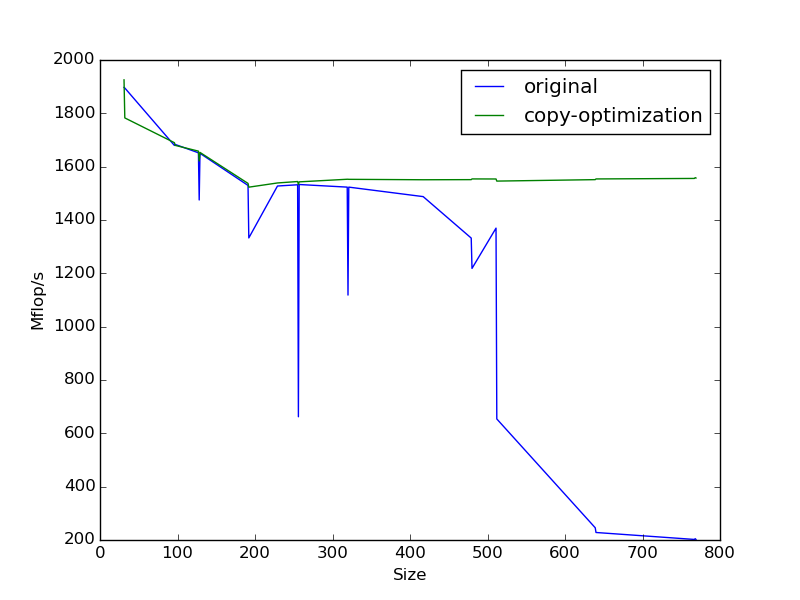
\includegraphics[width=0.6\textwidth]{figures/copy-optimization.png}
\caption{Difference in Mflop/s for (a) the original code and (b) the copy-optimization code that transposes \(A\).}
\label{fig:2}
\end{figure}

\subsection{SIMD Instructions}

\gls{simd} instructions allow a single instruction to be issued to perform an operation on multiple values at the same time. The registers on Edison each hold 32 bytes, which for double data type corresponds to four double values (8 bytes per double). Hence, there is potential for a four-fold improvement in speed, though likely the improvement will be lower because the program does not consist entirely of arithmetic operations such as adds and multiplies. The Ivy Bridge processor used in Edison uses \gls{avx} instructions, which through the {\tt immintrin.h} library allow access to a wide variety of methods to utilize \gls{simd} operations. The code below shows a simple implementation of \gls{simd} instructions in the naive code, where {\tt benchmark.c} has been modified to only include block sizes that are divisible by four (each register can only hold four double precision numbers). The transposed code from the previous section is used. To use \gls{simd} instructions in the blocked example for arbitrary matrix sizes, additional code will be written to account for block sizes that are not divisible by four.

\begin{lstlisting}[language=C, basicstyle=\small][H]
#include <stdlib.h>     // For: malloc
#include <immintrin.h>  // For: SIMD instrinsics

void square_dgemm (int n, double* A, double* B, double* C) {
  double * aij = 0;
  aij = (double*) malloc(n * n * sizeof(double));

  for (int i = 0; i < n; ++i) {
    for (int j = 0; j < n; ++j)
        aij[i + j*n] = A[j + i*n];
  }

  for (int i = 0; i < n; ++i) {
    for (int j = 0; j < n; ++j) {
      __m256d cij = _mm256_set1_pd(0);
      
      for(int k = 0; k < n; k+=4) {
        __m256d As = _mm256_load_pd(aij+k+i*n);
        __m256d Bs = _mm256_load_pd(B+k+j*n);
        cij += _mm256_mul_pd(As, Bs);
      }
      double tmp[4];
      _mm256_store_pd(tmp, cij);
      C[i+j*n] += tmp[0] + tmp[1] + tmp[2] + tmp[3];
  }}
  free(aij);
}
\end{lstlisting}

Fig. \ref{fig:6} shows the improvement in Mflop/s when using \gls{simd} instructions. As can be seen, there is more than a two-fold improvement in speed. For the blocked implementation, \gls{simd} instructions will be instrumental to obtaining as close to peak performance as possible. 

\begin{figure}[H]
\centering
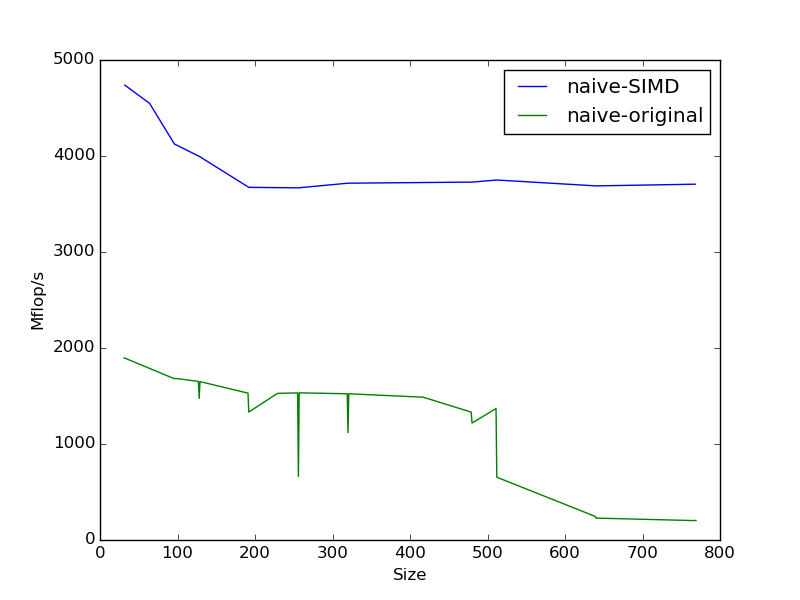
\includegraphics[width=0.6\textwidth]{figures/naive-original.png}
\caption{Difference in Mflop/s for (a) the code using \gls{simd} instructions with transposing {\tt A} (only shown for block sizes divisible by four) and (b) the original naive code.}
\label{fig:6}
\end{figure}

\subsection{Miscellaneous Optimizations}

% Talk about the compiler flags you guys played around with
% Talk about any results with/without restrict keyword
There are several other types of more minor optimizations that can be performed with the naive code. These include the use of the {\tt restrict} keyword and compiler flags. 

\section{Blocked Implementation}

This section discusses the optimizations performed with the blocked code ({\tt dgemm-blocked.c}), and takes advantage of lessons learned with the naive implementation to achieve fairly good performance for most matrix sizes.

\subsection{Column-Major Matrix Layout}
\label{sec:ColumnLayout}
This section discusses modifications to the blocked code that should permit fewer slow memory operations by improving spatial locality. Changing the layout of the matrices, as suggested by the great improvement in the results for large matrices in the naive implementation shown in Fig. \ref{fig:2}, can yield substantial increases in speed. Because the cache line size is greater than 1, fewer, or even simply a single, slow memory operation would be required to read in many matrix entries that are all then used in the same loop, avoiding repeated slow memory calls to the same data. The matrix layout should be optimized such that the cache line size reads in all necessary data, and hence the block size should be chosen to match the cache line size. This section discusses results obtained by re-structuring the \(A\) matrix, which is read in row-by-row, into a column-major format such that information is read in column-by-column. The code developed is shown below, where {\tt malloc} is used to dynamically allocate memory for the transformed matrix. This is implemented as a copy optimization, where \(A\) retains its original form, and \(a\) is the transposed matrix. \(A\) is transposed in the {\tt square\_dgemm} function and passed into the {\tt do\_block} function. This algorithm was further improved by removing the call to {\tt malloc} and instead assuming a sufficiently large size for the transposed matrix to work for all the test cases. Then, the matrix memory allocation is moved to compile-time, rather than run-time. However, this could fail for large matrix sizes. Fig. \ref{fig:3} shows the improvement associated with transposing \(A\) both with and without the use of {\tt malloc}.

\begin{lstlisting}[language=C, basicstyle=\small][H]
static void do_block (int lda,int M,int N,int K,double* A,double* B,double* C) {
  for (int i = 0; i < M; ++i) {
    for (int j = 0; j < N; ++j) {
      double cij = C[i+j*lda];
      for (int k = 0; k < K; ++k)
        cij += A[k + i*lda] * B[k+j*lda];
      C[i+j*lda] = cij;
  }}}

void square_dgemm (int lda, double* A, double* B, double* C) {
  double* a = 0;
  a = (double*) malloc(lda * lda * sizeof(double));

  for (int i = 0; i < lda; ++i) {
    for (int j = 0; j < lda; ++j)
        a[i + j*lda] = A[j + i*lda];
  }

  for (int i = 0; i < lda; i += BLOCK_SIZE) {
    for (int j = 0; j < lda; j += BLOCK_SIZE) {
      for (int k = 0; k < lda; k += BLOCK_SIZE) {
        int M = min (BLOCK_SIZE, lda - i);
        int N = min (BLOCK_SIZE, lda - j);
        int K = min (BLOCK_SIZE, lda - k);

        do_block(lda, M, N, K, a + k + i*lda, B + k + j*lda, C + i + j*lda);
  }}}
  free(a);
}
\end{lstlisting}

\begin{figure}[H]
\centering
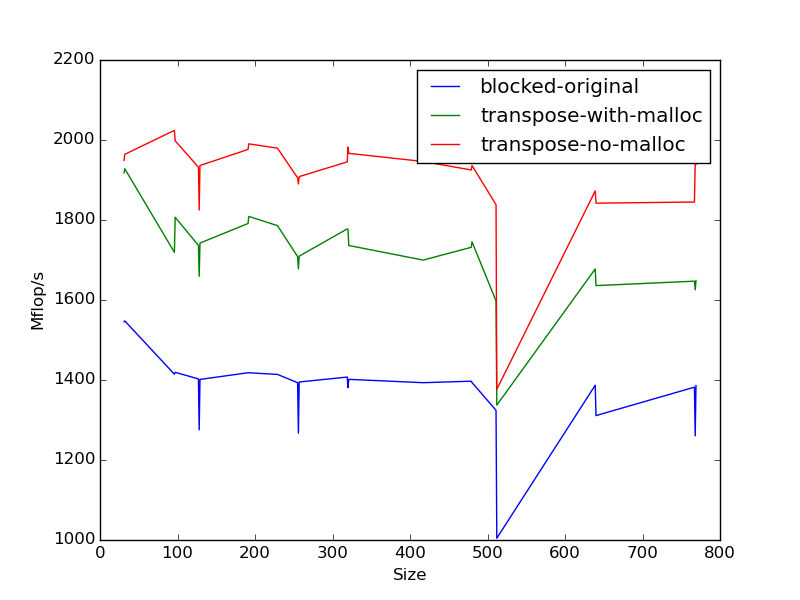
\includegraphics[width=0.6\textwidth]{figures/transpose-no-malloc.png}
\caption{Difference in Mflop/s for (a) the original blocked code, (b) the copy-optimization code that transposes \(A\) so that it can be accessed in a column-major layout using {\tt malloc}, and (c) the same copy optimization code that allocates a sufficiently large amount of memory for the transpose of \(A\).}
\label{fig:3}
\end{figure}
 
\subsection{Block Size}
This section discusses optimizations involving selection of the block size. First, using the column-layout code developed in Section \ref{sec:ColumnLayout}, block sizes in powers of 2 are tested to investigate if it is possible to learn what the cache line size of Edison is. Knowledge of the cache line size is useful because tailoring the code to seek data in chunks equal to the cache line size will reduce the number of cache misses. Fig. \ref{fig:4} shows the Mflop/s for various block sizes. It appears that a block size of 16 performs the best, though all sizes show a very clear drop in performance at a matrix size of 512\(\times\) 512, which is likely the size of the L2-cache. 
 
 \begin{figure}[H]
\centering
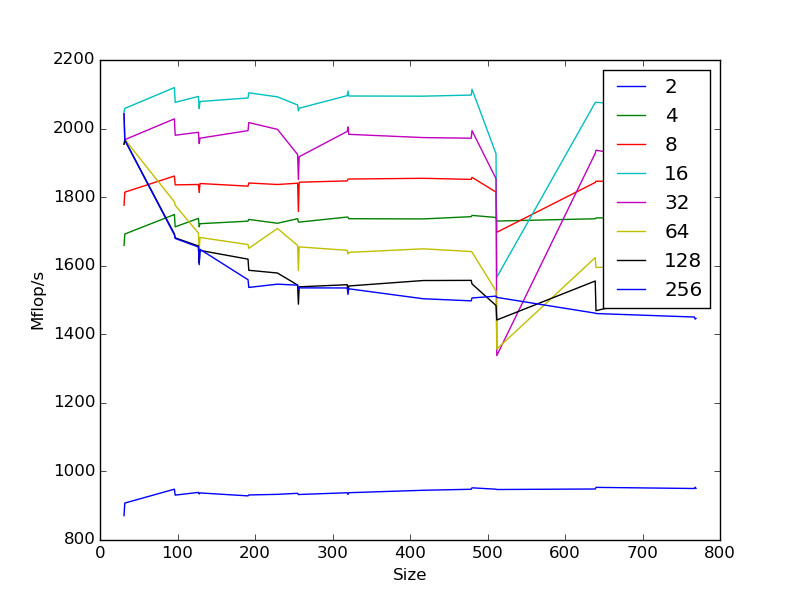
\includegraphics[width=0.6\textwidth]{figures/256.png}
\caption{Difference in Mflop/s for various block sizes, where the same block size is used for the \(i\) and \(j\) directions.}
\label{fig:4}
\end{figure}

Different block sizes can be used in each of the directions. Because {\tt C} uses a column-major format, it would likely be advantageous for the blocks to be more rectangular, with longer columns than rows. It appears from Fig. \ref{fig:5} that an optimal combination would be a block size of 16 in the {\tt i} direction and a size of 4 in the {\tt j} direction, though the improvement in using different block sizes is relatively small.

\begin{figure}[H]
        \centering
        \begin{subfigure}[b]{0.35\textwidth}
                \centering
                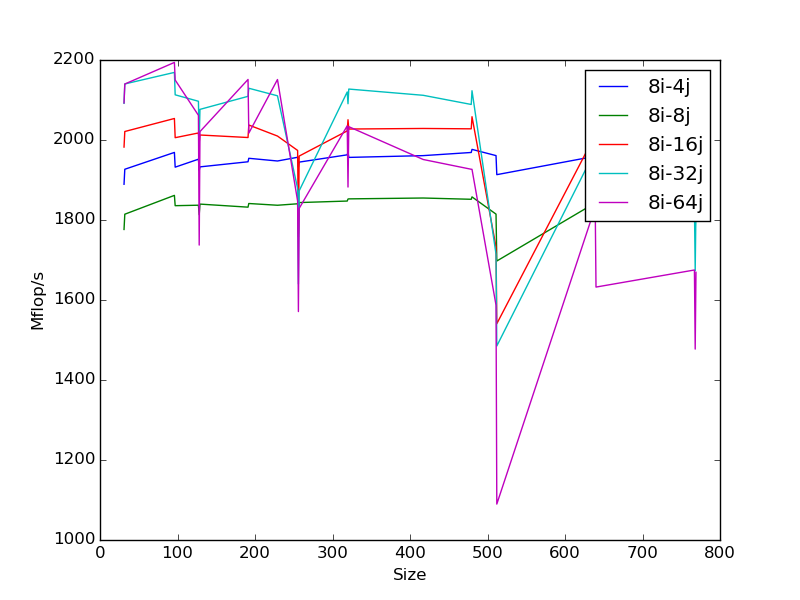
\includegraphics[width=\textwidth]{figures/8i-64j.png}
                \caption{{\tt BLOCK\_SIZE} 8 in {\tt i}}
        \end{subfigure}%
        \begin{subfigure}[b]{0.35\textwidth}
                \centering
                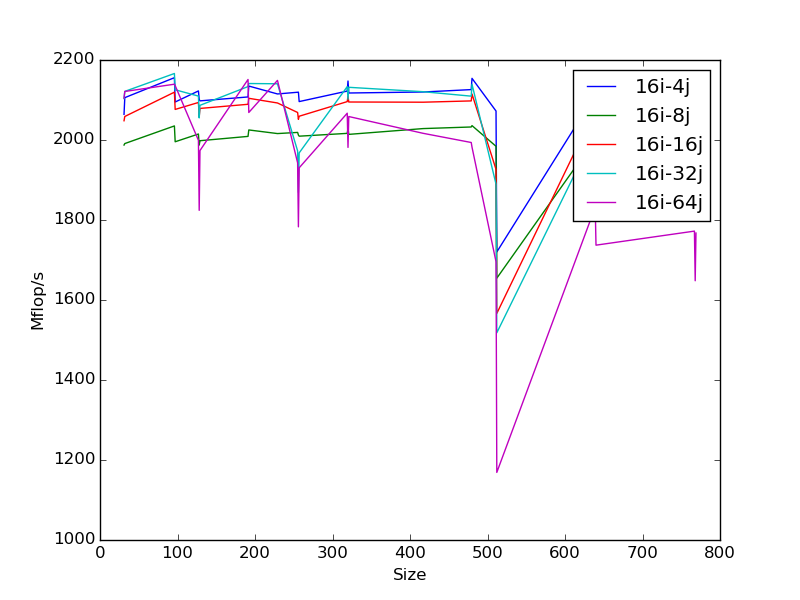
\includegraphics[width=\textwidth]{figures/16i-64j.png}
                \caption{{\tt BLOCK\_SIZE} 16 in {\tt i}}
        \end{subfigure}%
        \begin{subfigure}[b]{0.35\textwidth}
        \centering
        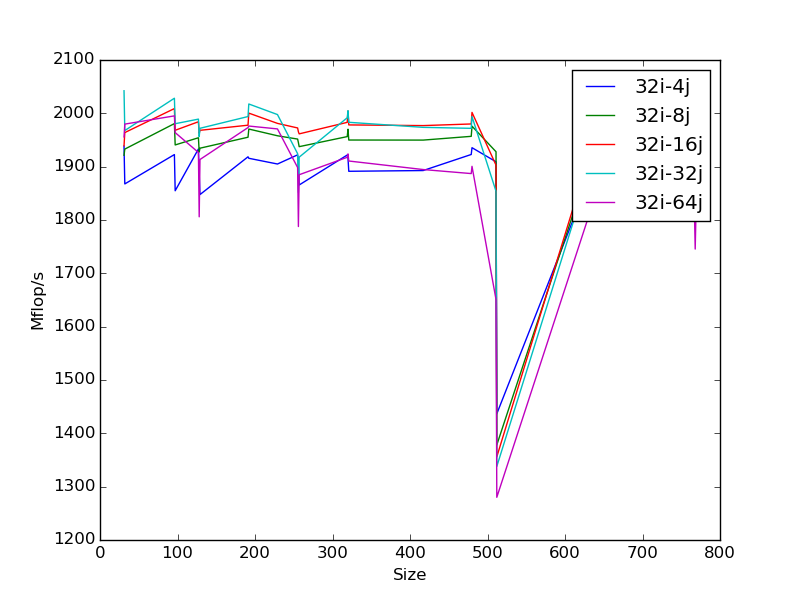
\includegraphics[width=\textwidth]{figures/32i-64j.png}
        \caption{{\tt BLOCK\_SIZE} 32 in {\tt i}}
        \end{subfigure}%
        \caption{Difference in Mflops for (a) 8, (b) 16, and (c) 32 {\tt BLOCK\_SIZE} in the {\tt i} direction for various sizes in the {\tt j} direction.}
        \label{fig:5}
\end{figure}

\subsection{SIMD Instructions} 

\section{Running the Optimized Code on Another Machine}

\section{Division of Work}

\end{document}
